\documentclass[uplatex,dvipdfmx,a4paper,twocolumn,base=11pt,jbase=11pt,ja=standard]{bxjsarticle}

\usepackage{ipsj}
\usepackage{color}
\usepackage{amssymb}

\title{チャネリング制約を用いた alldifferent 制約の SAT 符号化}{SAT Encoding of alldifferent Constraints with Channeling Constraints}
\author{名古屋大学}{小菅 脩司}{Shuji Kosuge, Nagoya University}
\author{神戸大学}{宋 剛秀}{Takehide Soh, Kobe University}
\author{神戸大学}{田村 直之}{Naoyuki Tamura, Kobe University}
\author{名古屋大学}{番原 睦則}{Mutsunori Banbara, Nagoya University}
\begin{document}
\maketitle

%%%%%%%%%%%%%%%%%%%%%%%%%%%%%%%%%%%%%%%%%%%%%%%%%%%%%%%%%% 
\chapter{序論}
\pagenumbering{arabic}
%%%%%%%%%%%%%%%%%%%%%%%%%%%%%%%%%%%%%%%%%%%%%%%%%%%%%%%%%% 

\textbf{ハミルトン閉路問題 (Hamiltonian Cycle Problem)} は,
与えられたグラフの全頂点をちょうど一度ずつ通る閉路が存在するかどうかを
判定する問題である.
\textbf{ハミルトン路問題 (Hamiltonian Path Problem)} は,
ハミルトン閉路問題から始点と終点が一致するという閉路の条件を取り除いた
ものである.
ハミルトン閉路問題とハミルトン路問題は,どちらも NP 完全な問題である.
これらの問題は,重要な工学的応用が数多く存在するため,古くから盛んに研
究されている.
例えば,数理最適化の分野で有名な巡回セールスマン問題は,グラフの辺に距
離が付随しているとき,最短距離のハミルトン閉路を求める
\textbf{最短ハミルトン閉路問題}と考えることができる.
また,ごく最近では,距離の総和が所与の閾値以下(または以上)であることを
制約条件として付加した
\textbf{コスト制約付きハミルトン閉路問題}\cite{comp20:Minato}
も提案されている.
本研究では,無向グラフ上のハミルトン閉路問題およびその関連問題を対象とする.

解集合プログラミング(Answer Set Programming; ASP)は,
論理プログラミングから派生した比較的新しいプログラミングパラダイムである.
ASP言語は,一階論理に基づく知識表現言語の一種であり,
論理プログラムは ASP のルールの有限集合である.
ASP システムは論理プログラムから安定モデル意味論に基づく解集合を計算す
るシステムである.
近年,SAT技術を応用した高速 ASP システムが開発され,スケジューリング,
プランニング,システム生物学,システム検証,制約充足問題,
制約最適化問題など様々な分野への実用的応用が急速に拡大している.
ハミルトン閉路問題およびその関連問題に対して ASP を用いる利点としては,
ASP 言語の高い表現力,
充足不能コアに基づく最適化,
インクリメンタルASP解法,
組込み非閉路制約,
高速な解列挙
などが挙げられる.

本論文では,解集合プログラミング(ASP)を用いた
ハミルトン閉路問題,
最短ハミルトン閉路問題,
コスト制約付きハミルトン閉路問題
の解法について述べる.
%
ハミルトン閉路問題を解くASP符号化として,
\textsf{undirected},
\textsf{directed},
\textsf{acyclicity}
の3つを考案した.
\textsf{undirected}は,
ハミルトン閉路問題を次数制約と部分閉路禁止制約で簡潔に表現した符号化である.
\textsf{directed}は,
与えられた無向グラフの各辺$u-v$に対して,
2つの弧$u\rightarrow v$と$v\rightarrow u$を対応させることで有向グラフ
化して解く符号化である.
変換した有向グラフ上のハミルトン閉路は元の無向グラフ上のハミルトン閉路
となり,また逆も成り立つ.
\textsf{acyclicity}は,\textsf{directed}符号化をベースに,
部分閉路禁止制約を組込み非閉路制約で表現した符号化である.
\textsf{acyclicity}符号化は,他の二つと比較して,基礎化後の制約数を少
なく抑えることができるため,大規模な問題に対する有効性が期待できる.
最短ハミルトン閉路問題とコスト制約付きハミルトン閉路問題については,
考案した3つの符号化に目的関数とコスト制約をそれぞれ追加することで自然に拡張できる.

考案した符号化の有効性を評価するために,
既存のベンチマーク問題集(7種類,計516問)を用いて実行実験を行なった.
その結果,
ハミルトン閉路問題とコスト制約付きハミルトン閉路問題(解の全列挙)について,
\textsf{acyclicity}符号化が,
\textsf{undirected}と\textsf{directed}と比較して,
より多くの問題を高速に解くことに成功し,その優位性を確認できた.
また,最短ハミルトン閉路問題については,
\textsf{undirected}符号化が,他の符号化と比較して,より多くの問題で最
適値・最良値を求めることができた.

%%% Local Variables:
%%% mode: latex
%%% TeX-master: "paper"
%%% End:

% \chapter{alldifferent 制約の SAT 符号化}
\section{alldifferent 制約の SAT 符号化}

%%% Local Variables:
%%% mode: latex
%%% TeX-master: "paper"
%%% End:

% \chapter{チャネリング制約を用いた alldifferent 制約の SAT 符号化}
\section{チャネリング制約を用いた alldifferent 制約の SAT 符号化}

順序符号化と直接符号化を組み合わせる際に用いた制約は以下の通りである.
$$p(x=a) \Leftrightarrow p(x \leq a) \land \lnot p(x \leq a)$$

チャネリングさせることで
順序符号化で有効な鳩の巣原理を用いたヒント制約や,
直接符号化で有効なat-least-one制約を組み合わせることができる.
alldiferent制約はPB・大野\cite{Ono19:ai}の手法で表現することができる.


\begin{table}[]
    \caption{提案した符号化一覧}
    \label{table:model}
    % {\scriptsize  \begin{tabular}[c] {|c|c|c|c|c|}\hline
  model & 符号    & alldiff & PHP & ALT1 \\\hline
  0     & OE      & neq     &    &      \\
  1     & OE      & neq     & \checkmark   &      \\
  2     & OE      & neq     &    & \checkmark    \\
  3     & OE      & neq     & \checkmark   & \checkmark    \\
  4     & OE{\textless=\textgreater}DE & neq     &    &  \\
  5     & OE{\textless=\textgreater}DE & neq     & \checkmark   &  \\
  6     & OE{\textless=\textgreater}DE & neq     &    & \checkmark \\
  7     & OE{\textless=\textgreater}DE & neq     & \checkmark   & \checkmark \\
  8     & OE{\textless=\textgreater}DE & PB      &    &   \\
  9     & OE{\textless=\textgreater}DE & PB      & \checkmark   &   \\
  10    & OE{\textless=\textgreater}DE & 大野3   &    &   \\
  11    & OE{\textless=\textgreater}DE & 大野3   & \checkmark   &   \\
  12    & OE{\textless=\textgreater}DE & 大野4   &    &   \\
  13    & OE{\textless=\textgreater}DE & 大野4   & \checkmark   &   \\\hline
 \end{tabular}
}
    {\tiny  \begin{tabular}[c] {c|c|c|c|c|c|c|c}
  符号化 & 整数変数の            & \multicolumn{4}{|c|}{alldifferent制
                                   約の表現} & PHP & ALT1 \\\cline{3-6}
        & 符号化法              & $\neq$分解 & 基本PB & PB3~\cite{Ono19:ai} & PB4~\cite{Ono19:ai} & & \\\hline
  0     & OE                    & OE      &    &       &             &     &      \\
  1     & OE                    & OE      &    &       &             & OE  &      \\
  2     & OE$\Leftrightarrow$DE & DE      &    &       &             &     &      \\
  3     & OE$\Leftrightarrow$DE & DE      &    &       &             &     & DE   \\
  4     & OE$\Leftrightarrow$DE & DE      &    &       &             & OE  &      \\
  5     & OE$\Leftrightarrow$DE & DE      &    &       &             & OE  & DE   \\
  6     & OE$\Leftrightarrow$DE &         & OE &       &             &     &      \\
  7     & OE$\Leftrightarrow$DE &         & OE &       &             & OE  &      \\
  8     & OE$\Leftrightarrow$DE &         &    & OE    &             &     &      \\
  9     & OE$\Leftrightarrow$DE &         &    & OE    &             & OE  &      \\
  10    & OE$\Leftrightarrow$DE &         &    &       & OE          &     &      \\
  11    & OE$\Leftrightarrow$DE &         &    &       & OE          & OE  &      \\\hline
 \end{tabular}
}
\end{table}
% % model.tex の説明
% 1列目は提案した符号化の番号を表している.
% 2列目は alldifferent 制約の符号化手法を表している.
% OE は順序符号化法で符号化することを表している.
% OE\textless=\textgreater DE は順序符号化法と直接符号化法をチャネリングさせて符号化する符号化することを表している.
% 3列目は alldifferent 制約の分解方法を表している.
% neq はnot-equal 制約に分解することを表している.
% PB はブール基数制約を用いて分解することを表している.
% 大野3・大野4は[大野,'19]の手法3・4を用いて分解することを表している.
% 4列目は 鳩の巣原理を用いたヒント制約の有無を表している.
% チェックマークを付けたモデルにヒント制約として追加している.
% 5列目は At-least-one 制約の有無を表している
% チェックマークを付けたモデルにヒント制約として追加している.

% model2.tex の説明
表\ref{table:model}は提案した alldifferent 制約のSAT符号化手法の一覧である.
1列目は提案した符号化の番号を,
2列目は 整数変数の符号化手法を表している.
OE は順序符号化法で符号化することを,
OE$\Leftrightarrow$ DE は順序符号化法と直接符号化法をチャネリングさせて符号化する符号化することを表している.
3列目は alldifferent 制約の分解方法を表している.
その中で$\neq$ はnot-equal 制約,
PB はブール基数制約,
大野3・大野4は[大野,'19]の手法3・4を用いて分解することを表している.
そして,どの分解方法を用いるのかと,それぞれの分解方法が直接符号化と順序符号化のどちらで符号化されるかをDEとOEで表している.
4・5列目は 鳩の巣原理を用いたヒント制約とat-least-one制約を直接符号化と順序符号化のどちらで符号化するのかとその有無を表している.




%%% Local Variables:
%%% mode: latex
%%% TeX-master: "paper"
%%% End:

%%%%%%%%%%%%%%%%%%%%%%%%%%%%%%%%%%%%%%%%%%%%%%%%%%%%%%%%%% 
\section{実行実験}\label{chap:experiment}
%%%%%%%%%%%%%%%%%%%%%%%%%%%%%%%%%%%%%%%%%%%%%%%%%%%%%%%%%% 

本章では,前章で提案した3つの符号化
\textsf{undirected},\textsf{directed},\textsf{acyclicity}
の性能を評価するために実行実験を行った.
%
実験に使用したベンチマーク問題集(計1008問)は,以下の通りである.
\begin{itemize}
\item \textsf{fhcp} (1001問)\\
  Jerzy Filar と Vladimir Ejov が主導する
  チームプロジェクト Flinders Hamiltonian Cycle Project
  \footnote{\url{https://sites.flinders.edu.au/flinders-hamiltonian-cycle-project/}}
  が提供するハミルトン閉路問題のグラフインスタンス.\cite{haythorpe19:fhcp}
\item \textsf{grid} (6問)\\
  $2N+1$次の正方グリッドグラフのインスタンス($3\leq N\leq 8$).
\item \textsf{usmap} (1問)\\
  図~\ref{fig:USmap}に示されたグラフ.
  D.~E~.Knuth の教科書
  The Art of Computer Programming~\cite{Knuth:TAOCP:SAT}
  に記載されている最短ハミルトン路問題の例.
\end{itemize}

使用した ASP システムは{\clingo}のバージョン5.5.0である.
実験環境は,Mac mini Intel Corei7 3.2GHz 64GBメモリである.

%%%%%%%%%%%%%%%%%%%%%%%%%%%%%%%%%%%%%%%%%%%%%%%%%%%%%%%%%%
\subsection{ハミルトン閉路問題の実験結果}
%%%%%%%%%%%%%%%%%%%%%%%%%%%%%%%%%%%%%%%%%%%%%%%%%%%%%%%%%%

%%%%%%%%%%%%%%%%%%%%%%%%%%%%%%%%%%%%%%%%%%%%%%%
\begin{table}[t]\scriptsize
  \centering
  %\tabcolsep = 0.8mm
  \renewcommand{\arraystretch}{1.2}
  \begin{tabular}{lr|rrr}
    問題サイズ & 問題数 & \textsf{undirected} & \textsf{directed} & \textsf{acyclicity}\\
   \hline
    $\:\:\:\:\:\,\, 0 \leq |V| < 1000$     & 171   & 156   & \alert{171}   & 156  \\ %
    $1000 \leq |V| < 2000$  & 165   & 120   & \alert{159}   & 121  \\
    $2000 \leq |V| < 3000$  & 177   & 125   & \alert{163}   & 80   \\
    $3000 \leq |V| < 4000$  & 185   & 104   & \alert{147}   & 48   \\
    $4000 \leq |V| < 5000$  & 128   & 92    & \alert{106}   & 30   \\
    $5000 \leq |V| < 6000$  & 80    & 63    & \alert{70}    & 21   \\
    $6000 \leq |V| < 7000$  & 55    & 39    & \alert{41}    & 20   \\
    $7000 \leq |V| < 8000$  & 28    & 12    & \alert{15}    & 4    \\
    $8000 \leq |V| < 9000$  & 10    & 2     & \alert{5}     & 1    \\
    $9000 \leq |V| < 10000$  & 2     & \alert{2}     & \alert{2}     & 1    \\
   \hline
    合計 & 1001 & 715   & \alert{879}   & 482  
  \end{tabular}
  \vskip .5em
%  \caption{ハミルトン閉路問題: 解けた問題数}
  \label{sat_table}
\end{table}
%label{sat_table}
%%%%%%%%%%%%%%%%%%%%%%%%%%%%%%%%%%%%%%%%%%%%%%%

%%%%%%%%%%%%%%%%%%%%%%%%%%%%%%%%%%%%%%%%%%%%%%%
\begin{figure}[tb]
\begin{center}
  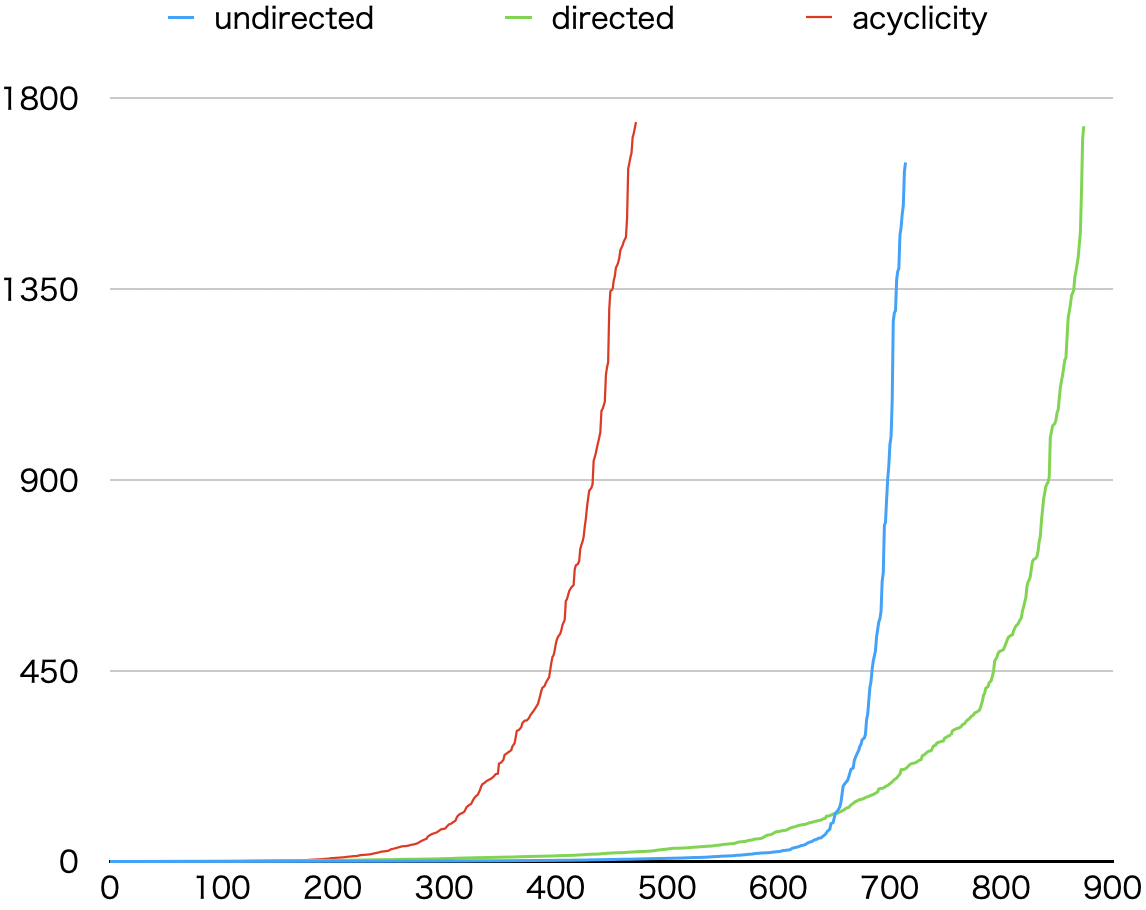
\includegraphics[width=0.8\linewidth]{fig/cactus_fhcp.png}
\caption{ハミルトン閉路問題: カクタスプロット}
\label{cactus}
\end{center}
\end{figure}
%%%%%%%%%%%%%%%%%%%%%%%%%%%%%%%%%%%%%%%%%%%%%%%


%--
本節では,ハミルトン閉路問題の実験結果について述べる.
{\clingo}のオプションは\textit{trendy}を使用し,一問あたりの時間制限を30分とした.
ベンチマーク問題は,\textsf{fhcp}の1001問である.

%--
表~\ref{sat_table}に,各符号化で解けた問題数を,問題の頂点数毎に示す.
左から,問題の頂点数,問題数,各符号化で解けた問題数を示している.
%
解けた問題数は,
\textsf{undirected}符号化が715問,
\textsf{directed}符号化が875問,
\textsf{acyclicity}符号化が473問であり,
\textsf{directed}がもっとも多くの問題を解いた.
\textsf{directed}は,どの頂点数においても同様に,
安定した性能の良さを示した.
図~\ref{cactus}に,カクタスプロットを示す.
縦軸は問題を解くのに要した CPU 時間,横軸は解けた問題数を表す.
グラフが右によるほど多くの問題を解けたことを示し,
下によるほどより速く解けたことを示す.
図~\ref{cactus}より,\textsf{directed}符号化が,
他の2つの符号化と比較して,より多くの問題を高速に解いていることが確認できた.
%% しかし,一部\textsf{undirected}符号化が\textsf{directed}符号化を下回る
%% 部分が確認できる.
%% 実際に,一部の問題では\textsf{undirected}符号化が
%% \textsf{directed}符号化よりも高速に解いていた.

%%%%%%%%%%%%%%%%%%%%%%%%%%%%%%%%%%%%%%%%%%%%%%%%%%%%%%%%%%
\subsection{最短ハミルトン閉路問題}
%%%%%%%%%%%%%%%%%%%%%%%%%%%%%%%%%%%%%%%%%%%%%%%%%%%%%%%%%%

%%%%%%%%%%%%%%%%%%%%%%%%%%%%%%%%%%%%%%%%%%%%%%%
\begin{table}[htbp]
  \caption{実験結果2-1:trendy}
  \label{min_table_tr}
  \centering
  \begin{tabular}{|l|rrr|}
    \hline
    Instance&undirected&directed&acyclicity \\
    \hline
    grid5&50,656*&50,656*&50,656* \\
    grid6&68,656*&68,656*&68,656* \\
    grid7&91,822*&91,822*&91,822* \\
grid8&113,250&\textcolor{red}{112,916}&113,277 \\
grid9&\textcolor{red}{142,502}&143,326&143,660 \\
grid10rc&\textcolor{red}{172,703}&174,866&175,999 \\
grid11&\textcolor{red}{200,399}&204,456&200,638 \\
grid12&\textcolor{red}{231,278}&239,275&232,012 \\
grid13&\textcolor{red}{276,692}&276,926&276,899 \\
grid14&317,617&\textcolor{red}{317,144}&317,676 \\
grid15&\textcolor{red}{375,906}&376,809&376,210 \\
grid16&421,249&\textcolor{red}{419,737}&423,753 \\
US48&11,698*&11,698*&11,698* \\
    \hline
  \end{tabular}
\end{table}
%\label{min_table_tr}
%%%%%%%%%%%%%%%%%%%%%%%%%%%%%%%%%%%%%%%%%%%%%%%

%--
本節では,最短ハミルトン閉路問題の実験結果について述べる.
{\clingo}のオプションは\textit{trendy}を使用し,
一問あたりの時間制限を3時間とした.
ベンチマーク問題は,\textsf{grid}と\textsf{usmap}の合計13問である.

%--
表\ref{min_table_tr}に,各符号化で得られた最適値と最良値を示す.
各問題毎に,最も良かった値を赤字で示している.
*マークは,最適値を表している.
最適値と最良値の数は,
\textsf{undirected}符号化が10問,
\textsf{directed}符号化が7問,
\textsf{acyclicity}符号化が4問であり,
\textsf{undirected}符号化の優位性が確認できた.

%%%%%%%%%%%%%%%%%%%%%%%%%%%%%%%%%%%%%%%%%%%%%%%%%%%%%%%%%%
\subsection{コスト制約付きハミルトン路問題}
%%%%%%%%%%%%%%%%%%%%%%%%%%%%%%%%%%%%%%%%%%%%%%%%%%%%%%%%%%

%%%%%%%%%%%%%%%%%%%%%%%%%%%%%%%%%%%%%%%%%%%%%%%
\begin{table*}[tb]\footnotesize
  \tabcolsep = 2mm
  %\renewcommand{\arraystretch}{1.0}
  \vskip .5em
  \centering
  \begin{tabular}{lr|rrr}
    \hline
    閾値(倍率)    &	解の総数 & \textsf{undirected} & \textsf{directed} & \textsf{acyclicity} \\
    \hline
    11698(1.00)   &	1      &\textbf{2.979} & 7.531 & 4.586	\\
    11814(1.01)   &	8      &5.587  & 15.322	& \textbf{5.250}	\\
    11931(1.02)   &	28     &\textbf{3.243}& 18.600	& 3.578	\\
    12282(1.05)   &	388    &10.003&19.818	& \textbf{6.296}	\\
    12867(1.10)   &	16,180  &16.548& 28.555	& \textbf{9.764}\\
    14037(1.20)   &	939,209 &48.262       &40.717	& \textbf{26.837}\\
    15207(1.30)   &	4,525,541&88.172      &55.276	& \textbf{42.037}\\
    16377(1.40)   &	6,702,964&99.154       &47.647	& \textbf{40.640}	\\
    17547(1.50)   &	6,876,526&95.390       &45.265	& \textbf{38.411}	\\
    18716(1.60)   &	6,876,928&98.937       &49.138	& \textbf{40.748}	\\
    \hline
    平均CPU時間 &   & 46.8275 & 32.7869  & \textbf{21.8147}\\\hline
%    Best    &   & 2 & 0 & \textbf{8} \\ \hline
  \end{tabular}
  \vskip .5em
  \caption{コスト制約付きハミルトン路問題: 解の全列挙に要した CPU 時間}
  \label{cost_table}
\end{table*}
%\label{cost_table}
%%%%%%%%%%%%%%%%%%%%%%%%%%%%%%%%%%%%%%%%%%%%%%%

%--
本節では,第~\ref{chap:background}章でも説明した
コスト制約付きハミルトン路問題(全列挙)の実験結果について述べる.
{\clingo}のオプションは\textit{crafty}を使用し,
一問あたりの時間制限を3時間とした.
ベンチマーク問題は,D.~E~.Knuth の教科書
The Art of Computer Programming~\cite{Knuth:TAOCP:SAT}
に記載されているグラフを使用した(図~\ref{fig:USmap}参照).
このグラフは,米国本土48州の隣接関係を表しており,
頂点数は48,辺の数は105である.
この問題の最短距離は 11698 である(表~\ref{min_table_tr}参照).
今回の実験では,
コスト制約を最短距離のN倍以下
($N=1.00,1.01,1.02,1.05,1.1,1.2,1.3,1.4,1.5,1.6$)として,解の全列挙を
行った.

%--
表~\ref{cost_table}に,各符号化が解の全列挙に要した CPU 時間を示す.
表の1列目はコスト制約の閾値と最短距離からの倍率,2列目は解の総数を表している.
各閾値毎に,最も良かった値を赤字で示している.
表より,
\textsf{acyclicity}符号化が,他の符号化と比較して,より多くの問題を
高速に解いていることがわかる.また,平均CPU時間も最も短い.
%%%%%%%%%%%%%%%%%%%%%%%%%%%%%%%%%%%%%%%%%%%%%%%%%%%%%%%%%%

%%% Local Variables:
%%% mode: latex
%%% TeX-master: "paper"
%%% End:

\chapter{おわりに}\label{chap:conc}

本論文では,電気制約として電流制約のみを考慮した配電網問題および配電網
遷移問題に対して,解集合プログラミング(ASP)を用いた解法を提案した.
配電網(遷移)問題に対する ASP を用いた研究は,著者らの知る限り,本論文
がはじめてである.
提案解法の特長と本論文の貢献について,以下にまとめる.

\begin{description}
\item[表現力:]
  配電網問題を解くための ASP 符号化を考案した.
  ASP 言語の高い表現力を生かし,
  配電網問題の制約を簡潔に記述できることを確認した.
  特に,有向符号化は,無向グラフの各辺$u-v$に対して,2つの弧
  $u\rightarrow v$と$v\rightarrow u$を対応させることで有向グラフ化して
  解く符号化であり,非閉路制約を簡潔に表現できる点が特長である.
\item[拡張性:]
  配電網遷移問題に対して,マルチショット ASP 解法を利用した符号化を提案した.
  この符号化は,配電網問題の ASP 符号化の自然な拡張となっている.
  マルチショット ASP 解法を利用することにより,
  ASP システムが同様の探索失敗を避けるために獲得した学習節を
  (部分的に)保持することで,無駄な探索を避けることができる点が特長である.
\item[効率性:]
  DNET (Power Distribution Network Evaluation Tool)
  に公開されている配電網問題(全3問)と,
  Graph Coloring and its Generalizations
  に公開されているグラフを基に独自に生成したトポロジ制約のみの配電網問
  題(計82問)を用いて実行実験を行なった.
  その結果,有向符号化は,他の2つの符号化と比較して,より多くの問題を
  より高速に解くことができ,その優位性を確認できた.
  %
  配電網遷移問題については,実用規模の問題({\sf fukui-tepco})に対して,
  実行可能解のペアをランダムに選び,合計 1000 問の配電網遷移問題を生成
  し,実行実験を行なった.その結果,すべての問題の到達可能性を判定する
  ことができ,得られた最短ステップ長の最大値は7であった.また,
  マルチショットASP解法を導入することにより,
  通常の解法と比較して,平均で3.8倍の高速化を実現した.
\end{description}

今後の課題としては,電流制約と電圧制約を含む完全な配電網問題への拡張が
挙げられる.しかし,完全な問題は非線形な制約を含むため,標準的な ASP
言語では記述できない.この問題を解決するために,近年研究開発が進められ
ている背景理論付き ASP (ASP Modulo Theories~\cite{DBLP:conf/iclp/GebserKKOSW16}) 
を用いた解法の実現可能性について調査を進める.

%%% Local Variables:
%%% mode: japanese-latex
%%% TeX-master: "paper"
%%% End:


\end{document}
